\documentclass[tikz]{standalone}
\tikzset{near start abs/.style={xshift=1cm}}

\usetikzlibrary{positioning}
\begin{document}
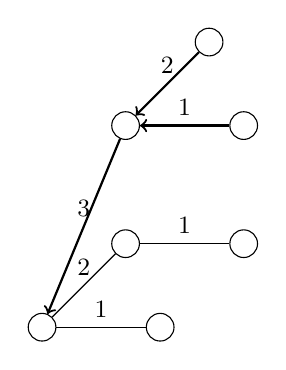
\begin{tikzpicture}[node distance=1.5cm]
    % place nodes
    \node[circle,draw=black, fill=white, inner sep=0pt,minimum size=10pt] (r) {};
    \node[circle,draw=black, fill=white, inner sep=0pt,right of=r, minimum size=10pt] (r1a)  {};
    \node[circle,draw=black, fill=white, inner sep=0pt,above right of=r, minimum size=10pt] (r2a)  {};
    \node[circle,draw=black, fill=white, inner sep=0pt,right of=r2a, minimum size=10pt] (r2b)  {};
    \node[circle,draw=black, fill=white, inner sep=0pt,above of=r2a, minimum size=10pt] (r3a)  {};
    \node[circle,draw=black, fill=white, inner sep=0pt,right of=r3a, minimum size=10pt] (r3b)  {};
    \node[circle,draw=black, fill=white, inner sep=0pt,above right of=r3a, minimum size=10pt] (r4a)  {};
    \draw (r) -- node[above] {\small{1}} ++(r1a);
    \draw (r) -- node[above] {\small{2}} ++(r2a);
    \draw[->,thick] (r3a) -- node[above] {\small{3}} ++(r);
    \draw (r2a) -- node[above] {\small{1}} ++(r2b);
    \draw[<-,thick] (r3a) -- node[above] {\small{1}} ++(r3b);
    \draw[<-,thick] (r3a) -- node[above] {\small{2}} ++(r4a);
\end{tikzpicture}
\end{document}